% Unofficial Umich Poster template.
% A fork of the MSU template https://www.overleaf.com/latex/templates/an-unofficial-poster-template-for-michigan-state-university/wnymbgpxnnwd
% which is a fork of https://www.overleaf.com/latex/templates/an-unofficial-poster-template-for-new-york-university/krgqtqmzdqhg
% which is a fork of https://github.com/anishathalye/gemini
% also refer to https://github.com/k4rtik/uchicago-poster

\documentclass[final]{beamer}

% ====================
% Packages
% ====================

\usepackage[T1]{fontenc}
\usepackage[utf8]{luainputenc}
\usepackage{lmodern}
\usepackage[size=custom, width=122,height=91, scale=1.2]{beamerposter}
\usetheme{gemini}
\usecolortheme{msu}
% Optional colors from YAML (main-color, title-color, header-color,
% text-color, accent-color), turned into LaTeX by poster.lua.
\definecolor{umichblue}{HTML}{00274C}
\definecolor{postertitle}{HTML}{00274C}
\setbeamercolor{block title}{fg=postertitle}
\setbeamercolor{block alerted title}{fg=postertitle}
\setbeamercolor{block example title}{fg=postertitle}
\definecolor{posterheader}{HTML}{00274C}
\setbeamercolor{headline}{bg=posterheader}
\definecolor{postertext}{HTML}{00274C}
\setbeamercolor{normal text}{fg=postertext}
\setbeamercolor{block body}{fg=postertext}
\setbeamercolor{block alerted body}{fg=postertext}
\setbeamercolor{block example body}{fg=postertext}
\setbeamercolor{heading}{fg=postertext}
\setbeamercolor{bibliography item}{fg=postertext}
\setbeamercolor{bibliography entry author}{fg=postertext}
\setbeamercolor{bibliography entry title}{fg=postertext}
\setbeamercolor{bibliography entry location}{fg=postertext}
\setbeamercolor{bibliography entry note}{fg=postertext}
\definecolor{posteraccent}{HTML}{FFCB05}
\setbeamercolor{block separator}{bg=posteraccent}
\setbeamercolor{block alerted separator}{bg=posteraccent}
\setbeamercolor{block example separator}{bg=posteraccent}
\usepackage{graphicx}
\usepackage{booktabs}
\usepackage{longtable}
\usepackage{array}
\usepackage{calc}
\usepackage{tikz}
\usepackage{pgfplots}
\pgfplotsset{compat=1.14}
\usepackage{anyfontsize}

% Support for pandoc-generated content (highlighting, tightlist, etc.)
\providecommand{\tightlist}{%
  \setlength{\itemsep}{0pt}\setlength{\parskip}{0pt}}
% Image sizing macro used by recent pandoc (\pandocbounded).
\makeatletter
\newsavebox\pandoc@box
\providecommand*\pandocbounded[1]{%
  \sbox\pandoc@box{#1}%
  \Gscale@div\@tempa{\textheight}{\dimexpr\ht\pandoc@box+\dp\pandoc@box\relax}%
  \Gscale@div\@tempb{\linewidth}{\wd\pandoc@box}%
  \ifdim\@tempb\p@<\@tempa\p@\let\@tempa\@tempb\fi%
  \ifdim\@tempa\p@<\p@\scalebox{\@tempa}{\usebox\pandoc@box}%
  \else\usebox\pandoc@box%
  \fi%
}
\makeatother

% ====================
% Lengths
% ====================

% If you have N columns, choose \sepwidth and \colwidth such that
% (N+1)*\sepwidth + N*\colwidth = \paperwidth
\newlength{\sepwidth}
\newlength{\colwidth}
\setlength{\sepwidth}{0.025\paperwidth}
\setlength{\colwidth}{0.3\paperwidth}

\newcommand{\separatorcolumn}{\begin{column}{\sepwidth}\end{column}}

% ====================
% Citations (citeproc); copied from Quarto's
% formats/beamer/pandoc/citations.tex, so [@key] citations and a
% ::: {#refs} ::: div work on the poster
% ====================

% definitions for citeproc citations
\NewDocumentCommand\citeproctext{}{}
\NewDocumentCommand\citeproc{mm}{%
  \begingroup\def\citeproctext{#2}\cite{#1}\endgroup}
\makeatletter
 % allow citations to break across lines
 \let\@cite@ofmt\@firstofone
 % avoid brackets around text for \cite:
 \def\@biblabel#1{}
 \def\@cite#1#2{{#1\if@tempswa , #2\fi}}
\makeatother
\newlength{\cslhangindent}
\setlength{\cslhangindent}{1.5em}
\newlength{\csllabelwidth}
\setlength{\csllabelwidth}{3em}
\newenvironment{CSLReferences}[2] % #1 hanging-indent, #2 entry-spacing
 {\begin{list}{}{%
  \setlength{\itemindent}{0pt}
  \setlength{\leftmargin}{0pt}
  \setlength{\parsep}{0pt}
  % turn on hanging indent if param 1 is 1
  \ifodd #1
   \setlength{\leftmargin}{\cslhangindent}
   \setlength{\itemindent}{-1\cslhangindent}
  \fi
  % set entry spacing
  \setlength{\itemsep}{#2\baselineskip}}}
 {\end{list}}
\usepackage{calc}
\newcommand{\CSLBlock}[1]{\hfill\break\parbox[t]{\linewidth}{\strut\ignorespaces#1\strut}}
\newcommand{\CSLLeftMargin}[1]{\parbox[t]{\csllabelwidth}{\strut#1\strut}}
\newcommand{\CSLRightInline}[1]{\parbox[t]{\linewidth - \csllabelwidth}{\strut#1\strut}}
\newcommand{\CSLIndent}[1]{\hspace{\cslhangindent}#1}

% ====================
% Title
% ====================

\title{Thirsty Engines: Why Your 1974 Car Hates Your Wallet}

\author{Jozef Rivest}

\institute[shortinst]{University of Michigan}

% ====================
% Footer (optional)
% ====================

\footercontent{
  \href{https://github.com/JozefRivest}{https://github.com/JozefRivest} \hfill
  Poster Session \hfill
  \href{mailto:jrivest@umich.edu}{jrivest@umich.edu}}

% ====================
% Logo (optional)
% ====================

% `logo` sets the image (path relative to the .qmd; default: blockM.png),
% `logo-height` its height (default: 5cm).
\logoright{
\includegraphics[height=5cm]{blockM.png}}

% ====================
% Body
% ====================

\begin{document}

\begin{frame}[t,fragile]
	\begin{columns}[t]

		\separatorcolumn

\begin{column}{\colwidth}

\begin{block}{Motivation}

Humanity's oldest question: \emph{why am I at the gas station again?}
Your uncle with the 1973 Cadillac has opinions. This poster has data
(Arel-Bundock 2025).

\end{block}

\begin{block}{Puzzle}

The Toyota Corolla gets \textbf{33.9} miles per gallon. The Cadillac
Fleetwood gets \textbf{10.4}. What is the Cadillac \emph{doing} with all
that gas?

\end{block}

\begin{block}{A bit of theory}

Two mechanisms explain engine thirst:

\begin{enumerate}
\def\labelenumi{\arabic{enumi}.}
\tightlist
\item
  \textbf{Many Mouths:} each cylinder is a tiny mouth that drinks
  gasoline
\item
  \textbf{Enthusiasm:} horsepower is \emph{how hard} those mouths drink
\end{enumerate}

\textbf{H1:} More cylinders mean fewer miles per gallon.

\textbf{H2:} Holding cylinders constant, more horsepower means fewer
miles per gallon.

\end{block}

\begin{block}{Background}

Lorem ipsum dolor sit amet, consectetur adipiscing elit. Sed do eiusmod
tempor incididunt ut labore et dolore magna aliqua. Ut enim ad minim
veniam, quis nostrud exercitation ullamco laboris nisi ut aliquip ex ea
commodo consequat.

Duis aute irure dolor in reprehenderit in voluptate velit esse cillum
dolore eu fugiat nulla pariatur. Excepteur sint occaecat cupidatat non
proident, sunt in culpa qui officia deserunt mollit anim id est laborum.

\end{block}

\begin{block}{Related work}

\begin{itemize}
\tightlist
\item
  Lorem ipsum dolor sit amet, consectetur adipiscing elit
\item
  Sed do eiusmod tempor incididunt ut labore et dolore
\item
  Ut enim ad minim veniam, quis nostrud exercitation
\item
  Duis aute irure dolor in reprehenderit in voluptate
\end{itemize}

Curabitur pretium tincidunt lacus. Nulla gravida orci a odio. Nullam
varius, turpis et commodo pharetra, est eros bibendum elit, nec luctus
magna felis sollicitudin mauris. Integer in mauris eu nibh euismod
gravida.

\end{block}

\begin{block}{Scope conditions}

Duis aute irure dolor in reprehenderit in voluptate velit esse cillum
dolore eu fugiat nulla pariatur. Excepteur sint occaecat cupidatat non
proident, sunt in culpa qui officia deserunt mollit anim id est laborum.

Lorem ipsum dolor sit amet, consectetur adipiscing elit. Sed do eiusmod
tempor incididunt ut labore et dolore magna aliqua. Ut enim ad minim
veniam, quis nostrud exercitation ullamco laboris nisi ut aliquip ex ea
commodo consequat.

\end{block}

\end{column}

\separatorcolumn

\begin{column}{\colwidth}

\begin{block}{Design}

I estimate the following model with OLS, because I know how to do it:

\[
\text{MPG}_i = \beta_0 + \beta_1 \text{Cyl}_i + \beta_2 \text{HP}_i + \varepsilon_i
\]

\end{block}

\begin{block}{Data}

\begin{itemize}
\tightlist
\item
  \texttt{mtcars}: 32 cars road-tested by \emph{Motor Trend} in 1974
\item
  Outcome: miles per gallon (higher = smugger)
\item
  Predictors: cylinders (mouths) and horsepower (enthusiasm)
\end{itemize}

\end{block}

\begin{block}{Results 1}

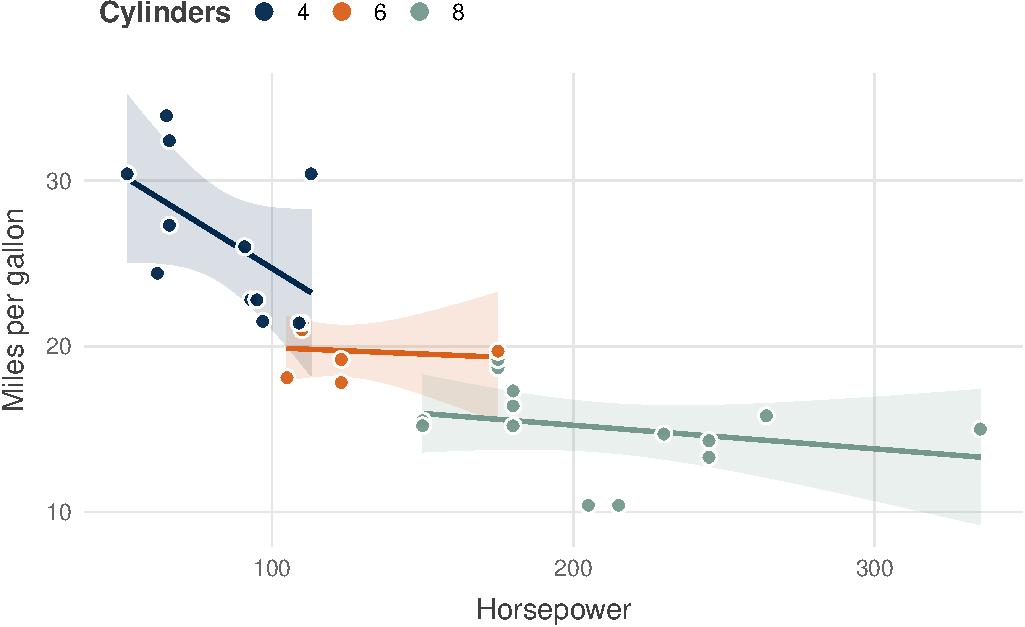
\includegraphics[width=1\linewidth,height=\textheight,keepaspectratio]{poster_files/figure-pdf/unnamed-chunk-1-1.pdf}

\end{block}

\begin{block}{Robustness}

Curabitur pretium tincidunt lacus. Nulla gravida orci a odio. Nullam
varius, turpis et commodo pharetra, est eros bibendum elit, nec luctus
magna felis sollicitudin mauris. Integer in mauris eu nibh euismod
gravida.

\begin{enumerate}
\def\labelenumi{\arabic{enumi}.}
\tightlist
\item
  Lorem ipsum dolor sit amet, consectetur adipiscing elit
\item
  Sed do eiusmod tempor incididunt ut labore et dolore magna
\item
  Ut enim ad minim veniam, quis nostrud exercitation ullamco
\end{enumerate}

Lorem ipsum dolor sit amet, consectetur adipiscing elit. Sed do eiusmod
tempor incididunt ut labore et dolore magna aliqua. Ut enim ad minim
veniam, quis nostrud exercitation ullamco laboris nisi ut aliquip ex ea
commodo consequat.

\end{block}

\begin{block}{Heterogeneity}

Duis aute irure dolor in reprehenderit in voluptate velit esse cillum
dolore eu fugiat nulla pariatur. Excepteur sint occaecat cupidatat non
proident, sunt in culpa qui officia deserunt mollit anim id est laborum.

\end{block}

\end{column}

\separatorcolumn

\begin{column}{\colwidth}

\begin{block}{Results 2}

\textbf{H1 confirmed:} an 8-cylinder car loses about 8.5 mpg relative to
a 4-cylinder car.

\begin{center}\LARGE

\begin{tabular}{lc}
\toprule
 & Model 1\\
\midrule
Constant & 28.650***\\
 & (1.588)\\
6 cylinders & -5.968**\\
 & (1.639)\\
8 cylinders & -8.521**\\
 & (2.326)\\
Horsepower & -0.024\\
 & (0.015)\\
Num.Obs. & 32\\
R2 & 0.754\\
\bottomrule
\end{tabular}
\end{center}

\end{block}

\begin{block}{Conclusion}

\begin{itemize}
\tightlist
\item
  More cylinders, fewer miles per gallon
\item
  \textbf{H2 runs out of gas:} horsepower is guilty in spirit, but
  \(p \approx 0.13\)
\item
  Future work: data from after 1974, and asking who \emph{needs} a V8
  for groceries
\end{itemize}

Vroom?

\end{block}

\begin{block}{Next steps}

Lorem ipsum dolor sit amet, consectetur adipiscing elit. Sed do eiusmod
tempor incididunt ut labore et dolore magna aliqua. Ut enim ad minim
veniam, quis nostrud exercitation ullamco laboris nisi ut aliquip ex ea
commodo consequat.

Curabitur pretium tincidunt lacus. Nulla gravida orci a odio. Nullam
varius, turpis et commodo pharetra, est eros bibendum elit, nec luctus
magna felis sollicitudin mauris. Integer in mauris eu nibh euismod
gravida.

\end{block}

\begin{block}{Acknowledgements}

Duis aute irure dolor in reprehenderit in voluptate velit esse cillum
dolore eu fugiat nulla pariatur. Excepteur sint occaecat cupidatat non
proident, sunt in culpa qui officia deserunt mollit anim id est laborum.

\end{block}

\begin{block}{References}

\protect\phantomsection\label{refs}
\begin{CSLReferences}{1}{1}
\bibitem[\citeproctext]{ref-arel-bundock25}
Arel-Bundock, Vincent. 2025. \emph{Model to Meaning: How to Interpret
Statistical Models with r and Python}. 1st ed. Chapman; Hall/CRC.
\url{https://doi.org/10.1201/9781003560333}.

\end{CSLReferences}

\end{block}

\end{column}

		\separatorcolumn
	\end{columns}
\end{frame}

\end{document}
